\section{Mixing time}\label{sec_mix}

Our first experiment will attempt to bound the mixing time of the Hit and Run random walk in a convex shape. The hit and run walk is known to mix rapidly~\cite{Lovasz98, Lovasz05} in the sense that the number of steps needed for the walk to approximate a uniform ditribution is $O^{*}(n^2)$, however this result actually shows that the walk can only be guaranteed to mix after over $10^{10} n^2$ steps. Performing $10^{10} n^2$ steps in a hit and run walk will take a very long time indeed, so if possible we would like to use far fewer.

We will generate 1,000 points with a hit and run walk using a variable number of steps, and perform a statistical test against a known uniform distribution to see if the walk has mixed properly. It is not clear which shape is likely to constitute a pathological case for the hit and run walk; the ice cream has the smallest volume, and so in a sense fewer points need to be chosen from, but also has the tighest possible corner, in which the walk is most likely to get stuck. By contrast, the ball has the largest volume and no corners. We will test both shapes. Uniformly distributed random points can be generated from a ball fairly easily, and uniform random points can be generated from an ice cream by simple rejection sampling. To keep our search reasonably short, we will restrict ourselves to only testing numbers of steps equal to natural powers of 2. Due to the extreme scaling of rejection sampling from an ice cream, it is not feasible to test any more than 8 dimensions on a home computer; though the wall clock times are not one of the variables we will be analysing, this information was still gathered for this experiment. If it took $t$ seconds to rejection sample 1,000 points from $n$ dimensions, then it took roughly $11t$ to sample the same number of points from $n+1$ dimensions. Points on a ball are still fairly easy to generate, and these could be tested up to 11 dimensions.

The analysis will use Ripley's K function~\cite{Dixon06}, a relatively modern and obsure statistical tool which summarises spatial point processes, allowing them to be compared easily. The K function does not uniquely define a process, but admits a measure of a process's distance from uniformity. The theoretical K function is defined as
$$
K(t) = \lambda^{-1}\mathbb{E}[\mbox{\# of extra points within distance $t$ of a randomly chosen point}]
$$
Where $\lambda$ is the density of events over the observed space -- the number of events per unit volume. The K-function is usually used for a process in 2 dimensional space, but generalises gracefully. For a perfectly uniform scattering of points, we have that
$$
K(t) = \vol_n(B)t^n
$$
To keep things consistent across dimensions, we will calculate values for the K function, then perform a simple transformation to produce the L function, defined
$$
L(t) = \left(\frac{K(t)}{\vol_n(B)}\right)^{\frac{1}{n}}
$$
So for a uniform scattering, we have that $L(t) = t$. Estimating $\lambda$ as $\widehat{\lambda}$ is fairly simple -- we divide the number of points seen by the volume of the space in which we see them -- estimating Ripley's K function naively for an observed sample is possible,
$$
\widehat{K}(t) =  \widehat{\lambda}^{-1} \sum_{\bm{u}} \sum_{\bm{v} \neq \bm{u}} \frac{\mathbb{I}(||\bm{u}-\bm{v}|| < t)}{N}
$$
Where $\mathbb{I}(x)$ takes the value of $1$ if $x$ is true, and $0$ otherwise. This naive estimate ignores edge effects - if a point is near to the edge of the study region, then we would expect fewer points to be nearby, so points near the edge shouldn't count for as much when estimating $K$. We neglect this edge correction here, since calculating it for complex high dimensional shapes is very difficult, and the error it leads to is systematic across the data for which $K$ functions are compared.

We will compute $\widehat{K}(t)$ for 100 values of $t$ evenly spaced between 0 and $\frac{v}{n}^{\frac{1}{n}}$, where $v$ is the volume of the region of interest, then convert it into its respective $\widehat{L}$. This function will be computed for points scattered by rejection sampling, our reference sample, and for a sequence of scatterings generated by a variable number of steps in the hit and run walk, our test samples. For two estimated $L$ functions, $\widehat{L}_1$ and $\widehat{L}_2$, we will consider the average absolute distance between $\widehat{L}_1$ and $\widehat{L}_2$. As the number of steps increases, the distance between the reference and test distributions will decrease to some small value. When the average absolute distance appears to stop decreasing, we will judge the walk to be well-mixed -- at this point increasing the number of steps cannot be expected to bring the distributions any closer.

\begin{figure}
\centering
\subfigure[An example estimated $L$ function for scattering in a 5-dimensional ice cream -- a $2^1$-step random walk against the reference rejection sampling method. Note that the functions are very different for this small number of steps.]{
	\includegraphics[width = 0.4 \textwidth]{./images/ice_cream_5-dimensions_1-steps.pdf}
}
\subfigure[An example estimated $L$ function for scattering in a 5-dimensional ball -- a $2^1$-step random walk against the reference rejection sampling method.]{
	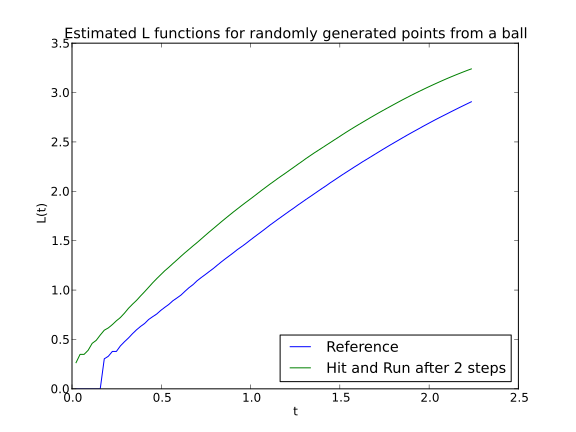
\includegraphics[width = 0.4 \textwidth]{./images/ball_5-dimensions_1-steps.pdf}
}
\\
\subfigure[An example estimated $L$ function for scattering in a 5-dimensional ice cream -- a $2^{10}$-step random walk against the reference rejection sampling method. Note that increasing the number of steps has caused the functions to become very similar.]{
	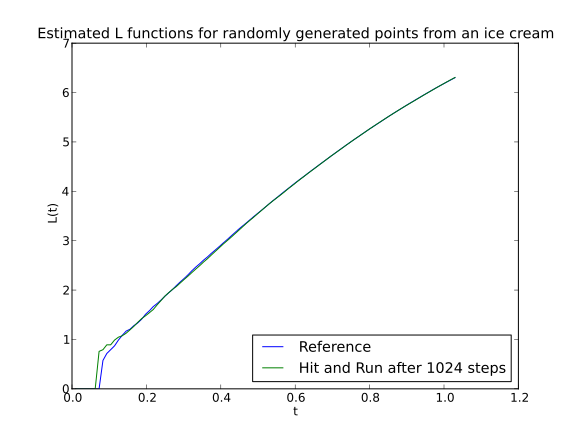
\includegraphics[width = 0.4 \textwidth]{./images/ice_cream_5-dimensions_10-steps.pdf}
}
\subfigure[An example estimated $L$ function for scattering in a 5-dimensional ball -- a $2^{10}$-step random walk against the reference rejection sampling method.]{
	\includegraphics[width = 0.4 \textwidth]{./images/ball_5-dimensions_10-steps.pdf}
}
\\
\subfigure[The average distances for tests on a 5 dimensional ice cream. Note that the average distance stops changing significantly and remains small after, in this case, $2^4$ steps]{
	\includegraphics[width = 0.4 \textwidth]{./images/ice_cream_5-dimensions.pdf}
}
\subfigure[The average distances for tests on a 5 dimensional ball.]{
	\includegraphics[width = 0.4 \textwidth]{./images/ball_5-dimensions.pdf}
}
\caption{Graphs of $L$ functions, and the distances between them}
\label{fig_steps}
\end{figure}

Large quantities of data were generated, so~\ref{fig_steps} only shows a small number of results. The conclusion from inspecting all of the graphs is that using at least $2^5$ steps reliably produces random points of good quality, and also that neither shape represented a particularly pathological case. Given the difficulty of taking a hit and run step, this is still a relatively expensive random number generator, but nowhere near the theoretical bound of $10^{10}$. This is relieving, and we will use these 32 steps in the random walk for the following experiments.

Running gprof over the code as it executes reveals that roughly 60\% of the time for each random walk is spent executing the binary search to find the boundaries of the convex shape, and even a simple oracle such as one for the ball $RB$ consumes another 20\% of the walk time. If further work is to be performed on the algorithm, authors may be well advised try and control this time.

\section{Threads per stage}\label{sec_error}

We will now see how the number of threads per phase influences the accuracy of an estimate. In the paper describing our particular estimation method, it is stated that, for an n-dimensional shape, in order to achieve an error of $\varepsilon$, we should use $400\frac{n\log n}{\varepsilon^2}$ threads per stage. This, again, is an upper bound, and we would like to show that it is loose. We shall vary the number of threads used per stage, and see how the distribution of estimates varies with this value. As before, we will use both the ice cream and the ball to respectively maximise and minimise the ratios between successive shapes. Our analysis here will be largely visual, since any returned value from this algorithm might be considered valid for a sufficiently large value of epsilon.

In all cases the errors decrease fairly rapidly, with estimates being easier to acquire for the ball than for the ice cream. The ice cream is very much the pathological case here. These figures can be used to read off the minimum number of threads needed to get an estimate of a given quality, but it is interesting to note that estimates show a clear tendency to converge towards slightly incorrect values. It is possible that this convergence is due to numerical instability. Note that an inverse polynomial relationship with $\varepsilon$ remains apparent in the graph of greatest absolute error.

We also depict the greatest errors made on each shape in terms of apsolute error. Because of the vast number of graphs, figure~\ref{fig_histograms} will only show a few.

\begin{figure}
\centering
\subfigure[Histograms for the ball estimates]{
	\includegraphics[width = 0.4 \textwidth]{./images/6-dimensions_ball_3d.png}
}
\subfigure[Histograms for the ice cream estimates]{
	\includegraphics[width = 0.4 \textwidth]{./images/6-dimensions_ice_cream_3d.png}
} 
\\

\subfigure[The worst mistakes made in the ball estimates]{
	\label{fig_2d_ball}
	\includegraphics[width = 0.4 \textwidth]{./images/6-dimensions_ball_2d.pdf}
}
\subfigure[The worst mistakes made in the ice cream estimates]{
	\includegraphics[width = 0.4 \textwidth]{./images/6-dimensions_ice_cream_2d.pdf}
	\label{fig_2d_ice_cream}
}
\caption{Variance in errors for various shapes, measured in different ways}
\label{fig_histograms}
\end{figure}

So, reading off from figures~\ref{fig_2d_ice_cream} and~\ref{fig_2d_ball}, in a 6-dimensional ice cream our estimates all become correct for $\varepsilon > 0.1$ for any number of threads greater than $2^11 = 2,048$. For a 6-dimensional ball to within an error of $0.1$, we need more like $2^{13} = 8,192$. In all cases, the error drops below $0.2$ for $2^{13}$ threads per stage. To achieve an accuracy of 0.2 in 11 dimensions, the papers suggest that at least $400\frac{n\log n}{\varepsilon^2} \approxeq 380,000$ threads are necessary for each stage. Once again, the bound is very loose indeed.

\section{Computation Time for Convex Shapes}\label{sec_time}

It's now time to test the practicalities of this algorithm on a series of convex shapes, against already established methods of exact volume computation. The code used for comparison is the same as that used in~\cite{Bueler98}
and was run over a series of randomly generated convex shapes. We will randomly generate series of shapes in each dimension and see how this affects the time for a volume estimation to complete using the values found above by experimentation

All experiments were conducted on the same hardware and on the same operating system, using the same time metric. The processor is an Intel i5-2500k in a Gigabyte Z68AP-D3 motherboard, connected to 8 GiB of 1,600 MHz dual-channel DDR3 RAM. The programs were both compiled onto a 64-bit install of Ubuntu 12.04 virtualised by Oracle VM Virtualbox with access to 2GiB of RAM using gcc. Each time is measured in elapsed clock cycles divided by the number of clocks per second. Using this processor time removes the possibility of error due to other running processes. The actual wall-clock time is significantly longer, but the listed times ignore the time spent by the OS performing other processes, as well as the overhead incurred for virtualisation. Neither program is designed to exploit any more than a single processor core, since to ensure a fair comparison we would require extensive modification of the code from~\cite{Bueler98}.

Initially, the oracle was implemented with a linear programming solver. A point ${\bm p}$ lies within the convex hull of a set of $v$ vertices $\{{\bm x}^1, {\bm x}^2, {\bm x}^3, ..., {\bm x}^v\}$ iff there exists a vector ${\bm \lambda}$ such that

\begin{align*}
\lambda_1 x^1_1 + \lambda_2 x^2_1 + ... + \lambda_v x^v_1 &= p_1 \\
\lambda_1 x^1_2 + \lambda_2 x^2_2 + ... + \lambda_v x^v_2 &= p_2 \\
&\vdots \\
\lambda_1 x^1_n + \lambda_2 x^2_n + ... + \lambda_v x^v_2 &= p_n \\
\lambda_1 + \lambda_2 + ... + \lambda_v &= 1
\end{align*}

This defines the feasible region of an LP problem, which an LP solver can then inspect to see if any solutions for ${\bm \lambda}$ exist. The solver used was Gurobi, chosen simply because it is the fastest availalbe LP solver. Whilst the LP solver is fast, it will be given vast numbers of LPs to solve, leading to some slow execution times.

This particular method of representing a polytope is known as vertex representation, or v-representation. It is also possible to represent a polytope as two sets of halfspaces. A point lies in a convex polytope iff it is below some set of halfspaces and above some other set of halfspaces. Each halfspace forms one facet of the polytope. Representing a polytope as a set of halfspaces is known as the h-representation. The fastest exact methods require the shape to be converted from v-representation to h-representation before the volume can be computed. Facet enumeration, the problem of performing this computation, is solvable in $O(vl(v,n)f)$ time\cite{Fukuda97}, where $f$ is the eventual number of facets, and $l(v,n)$ is the complexity of solving a linear programming problem in $n$ variables and $v$ constraints. LP solving is exponential in its worst case~\cite{Klee72}, but is known to be efficient when used against real-world problems. The number of facets on each randomly generated polytope tends to be very large, see table~\ref{tab_num_facets}.

Generating a large sample size across several dimensions and several shapes would be time-consuming. Where previously we could comfortably generate thousands of data points, here we will have to restrict ourselves to 5 samples from each experiment. In each experiment, we will start with the $n$-dimensional cross-polytope $\{{\bm x} | \sum^n_{i=1}|x_i| \leqslant R\}$, add either 0, 25, 50, 75 or 100 extra vertices, uniformly distributed over the surface of the ball of radius $R$, then estimate the volume of their convex hull. From the definition of the cross-polytope, it is fairly easy to show that it is exactly the convex hull of the points $\pm R{\bm e}_i$ for $i \in \{1,2,...,n\}$, where ${\bm e}_i$ is the vector whose $i^{th}$ component is 1, and all others are 0, so each cross-polytope adds exactly $2n$ vertices to the v-representation. Since $R=\sqrt{n}$, this cross-polytope always contains the unit ball, see Appendix~\ref{app_cross_polytope}. 

Starting with this cross polytope is a simple solution to what is actually a rather complicated problem. It is, in fact, very difficult to check that a randomly generated polytope contains the unit ball, a condition which is required for the estimation technique to make sense. We will take a short diversion to explain why this is the case.

\begin{proposition}
Let ${\bm x}_1, ..., {\bm x}_v$ be a sequence of $v$ vertices selected uniformly at random from the surface of an $n$-ball of radius $R>1$. The problem of determining whether their convex hull contains the unit ball is NP-hard in either direction, assuming NP $\neq$ co-NP.
\end{proposition}

Note that we cannot simply perform facet enumeration on each of our vertices and check that the distance from the origin to the hyperplane representing each facet is less than one. From the results in appendix~\ref{app_cyclic_polytope}, even with a linear number of vertices, we can construct a shape with an exponential number of facets.

It's fairly easy to see that showing the ball is not within the hull is in NP. Given our set of points, I can produce a polynomial certificate to prove that their hull does not contain the unit ball by providing a point $\bm p$ on the surface of the unit ball that is not contained within their hull. We can then check that $||\bm{p}|| = 1$ and that the convex hull of ${\bm x}_1, ..., {\bm x}_v$ does not contain $\bm p$ by standard linear programming. If this fails, the convex hull cannot contain the unit ball.

$\bm p$ exists if and only if there exists some separating hyperplane such that ${\bm x}_1, ..., {\bm x}_v$ and the point $(0,0,...,0)$ lie on the same side of the hyperplane, and the distance from the origin to the hyperplane is less than one. If this separating hyperplane exists, then we know that the convex hull of ${\bm x}_1, ..., {\bm x}_v$ must lie on  one side of the hyperplane, and there is a point $\bm p$ on the other side of the hyperplane with $||\bm{p}|| = 1$, which must lie outside of the convex hull. Conversely, if every such hyperplane must be further from the origin than 1, then any point $\bm p$ outside this hull must satisfy $||\bm{p}||>1$. The problem of determining whether a convex hull contains the unit ball reduces to the problem of finding a separating hyperplane of distance less than 1 from the origin.

A plane can be defined as the set of points $\{ {\bm x} \in \arr ^n | \sum^n_{i=1} a_i x_i = 1\}$, for some vector ${\bm a} \in \arr ^n$. The distance from this plane to the origin is $\frac{1}{||{\bm a}||}$, and the two sides of the hyperplane are the sets $\{ {\bm x} \in \arr ^n | \sum^n_{i=1} a_i x_i > 1 \}$ and $\{ {\bm x} \in \arr ^n | \sum^n_{i=1} a_i x_i < 1 \}$. The notions of ``above" and ``below" are arbitrary, since we can replace $\bm a$ with $-\bm{a}$ to switch these two sets over. We can state this separating hyperplane problem as finding a point ${\bm a} \in \arr^n$ such that
\begin{align*}
\forall i \in \{1, ..., v\} \; \; {\bm a} \cdot {\bm x}_i &\leqslant 1 \\
||{\bm a}|| &> 1
\end{align*}
This problem then reduces to solving the following quadratic programming problem:
\begin{align*}
\mbox{Minimise: }& f({\bm a}) = {\bm a}^T (-I) {\bm a} \\
\mbox{Subject to: }& i \in \{1, ..., v\} {\bm a} \cdot {\bm x}_i \leqslant 1 
\end{align*}
Where $I$ is the identity matrix and ${\bm a}^T$ is the transpose of ${\bm a}$ -- ${\bm a}$ written as a row vector. $-I$ has at least one negative eigenvalue and so, from the results of a didactically-named paper by Pardalos and Vavasis~\cite{Pardalos91}, solving this problem is NP-Hard. The forward problem is NP-hard, and the reverse problem is in NP. Therefore, assuming NP $\neq$ co-NP, both the forward and reverse problems are NP-hard.

This means that there is no efficient way to test whether or not the points we have chosen contain the unit ball. Not only this, but we can also show that the probability these points contain the unit ball is low.

\begin{proposition}
The probability that the origin is contained within the convex hull of $v$ vertices chosen uniformly at random from the surface of an origin-centred ball is no more than $\frac{1}{2}$ when $v = 2n$.
\end{proposition}

J. G. Wendel~\cite{Wendel62} evaluated the probability that a set of $v$ vertices selected uniformly on the surface of an $n$-ball all lie on the same hemisphere. This condition is equivalent to the origin being containined within their convex hull. This probability, $p_{n,v}$, is defined

$$
p_{n,v} = 2^{-v+1} \sum_{k=0}^{n-1} {{v-1} \choose k}
$$

The sum of the elements of the $v-1^{th}$ row of Pascal's triangle is $2^{v-1}$~\cite{mathworld_pascal}. If we choose $v = 2n$, then $v-1$ is odd, and the $v-1^{th}$ row has $v$ entries. Because the rows are symmetric, summing up the first $n-1$ entries of the $v-1^{th}$ row gives us a value no greater than $2^{v-2} = 2^{2n-2}$, so $p_{n, 2n} \leqslant 2^{2n+1} 2^{2n-2} = \frac{1}{2}$.

If the hull contains the unit ball, it must also contain the origin, so the probability that the hull contains the unit ball is bounded above by the probability that it contains the origin. We need more than $2n$ points to ensure that the hull contains the origin with probability greater than $\frac{1}{2}$, so we may as well choose $2n$ points to begin with which we know for certain will contain the unit ball.

The data for each generated shape will be passed into an exact solver, which will attempt to convert the shape from its v-representation to an h-representation, then compute the exact volume via the Hybrid Orthomormalisation Technique~\cite{Bueler98}. If any stage takes longer than one hour of processor time, it will be terminated early. The number of the experiment will be used as a random number seed; the Mersenne Twister will be seeded from 1, 2, 3, 4, and 5, depending on the experiment, and the Ziggurat will be seeded from a number generated by the Mersenne Twister. Anything that remains unclear can hopefully be explained by reading the code. %cite code

\begin{table}[h]
\centering
\begin{tabular}{| c || p{1cm} | p{1cm} | p{1cm} | p{1cm}|}
\hline
&\multicolumn{4}{p{5cm}|}{Average Computation Time for $v$ Extra Points (minutes)} \\
\hline
Number of Dimensions & $v$=25 & 50 & 75 & 100\\
\hline
8  & 20 & 25 & 27 & 36 \\
9  & 24 & 29 & 38 & 41 \\
10 & 28 & 37 & 43 & 54 \\
\hline
\end{tabular}
\caption{Average Computation Times for Volume Estimation}
\label{tab_estimation_time}
\end{table}

\begin{table}[h]
\centering
\begin{tabular}{| c || p{1cm} | p{1cm} | p{1cm} | p{1cm}|}
\hline
&\multicolumn{4}{p{5cm}|}{Average Number of Facets for $v$ Extra Points} \\
\hline
Number of Dimensions & $v$=25 & 50 & 75 & 100\\
\hline
8  & 10,826 & 34,827  & 69,713  & 110,412 \\
9  & 28,662 & 114,267 & 249,243 & $\bot$ \\
10 & 78,534 & $\bot$ & $\bot$ & $\bot$ \\
\hline
\end{tabular}
\caption{Average Number of Facets for shapes generated in $n$ dimensions. Numbers of $\bot$ denote a failed calculation, since the facet enumeration timed out before a value could be found.}
\label{tab_num_facets}
\end{table}

\begin{table}[h]
\centering
\begin{tabular}{| c || p{1cm} | p{1cm} | p{1cm} | p{1cm}|}
\hline
&\multicolumn{4}{p{5cm}|}{Average Conversion Time for $v$ Extra Points (minutes)} \\
\hline
Number of Dimensions & $v$=25 & 50 & 75 & 100\\
\hline
8 & 0   & 1      & 4      & 11 \\
9 & 0   & 6      & 38     & $\bot$ \\
10& 6   & $\bot$ & $\bot$ & $\bot$ \\
\hline
\end{tabular}
\caption{Average Times to convert from v-representation to h-representation. Times of $\bot$ denote a conversion which was timed out for taking more than an hour.}
\label{tab_conversion_time}
\end{table}

Inspecting all values suggests a linear scaling across both axes for the estimation times, and exponential scaling across both axes for the conversion times from v-representation to h-representation. Tables~\ref{tab_estimation_time} and~\ref{tab_conversion_time} show the interesting sections of the results. This scaling isn't entirely unexpected -- we already know that the shape will always have an exponential number of facets with respect to $n$, and for shapes more complex than 50 points in 10-dimensional space the time to convert from v to h representation is significantly longer than the time to simply estimate the shape's volume via the monte-carlo techniques. Indeed, in one of the preliminary experiments, a shape with $n=10$ and $v=100$ was input into the conversion code for an evening. After 6 hours, the output reported that it had completed $75\%$ of its iterations. Each iteration appeared to take longer than the previous one, but the code will have needed at least 8 hours in total to complete the conversion. Compare this to the 53 minutes needed to estimate one of these volumes to within a reasonable degree of accuracy.

After the conversion, the times to compute volumes are barely worth reporting. The longest time across all shapes was achieved for $n=9$ and $v = 75$, taking around 5 minutes -- negligible in comparison to the 38 minutes taken for conversion, a trend which continued for all the generated shapes.

\section{Conclusions and Future Work}

Given a vertex representation for a convex shape in $n$ dimensions, using exact methods to compute its volume remains a viable option for $n<9$ and a reasonably simple shape, however as the number of dimensions grows beyond this, it becomes highly impractical to continue with exact methods, and monte-carlo based volume estimation becomes a very attractive option indeed. The specific parameters needed for these operations are generally significantly lower than those theorised, meaning that significant savings can be made for a practical implementation.

However, a convex shape in $10$ dimensions with $120$ vertices is still fairly simple, yet requires roughly an hour of processor time to process. Even estimating the volume of a convex shape is very difficult, and these methods do not provide a substitute for domain specific knowledge and careful consideration of the shapes at hand.

Some questions remain unanswered by this study. These shapes were deliberately chosen to fulfil the properties required by the volume estimation algorithms, however any shape can be transformed to fulfil these properties by sampling a large number of points uniformly, then transforming these such that they contain the unit ball and are contained within a ball of fixed radius. These methods were simply untested in this study, but there are probably also useful experimental results on the number of points necessary to transform a shape ``well". With more computational power, more data points could be generated leading to more information on how these methods scale into more dimensions - a supercomputer cluster could easily generate data for shapes in several hundred dimensions, but these data had to be gathered from a single home computer. It would also be interesting to see how well these methods could be parallelised - each random walk can certainly be simulated independently of all others, so it would probably be possible to scale these methods up to some very large clusters.

We also still have little knowledge of the properties of a randomly generated convex shape. What, on average, is its volume? How can we randomly generate one which definitely contains the unit ball, but also has a reasonable number of facets? The method used here produces a randomly generated convex shape whose vertices are all a fixed distance from the origin. What would happen if we also allowed the distance to vary?

Comparing distributions in $n$ dimensions also remains largely unsolved. The techniques used in Section~\ref{sec_mix} were fairly crude, and I can find no authors who have tried to extend Ripley's K function into $n>2$ dimensions, nor any who can provide $p$ values for significance testing for anything other than a few very specific cases. Comparing distributions of random vectors would be a very useful tool indeed when analysing multivariate data.

To finish, the appendices will investigate various subsidiary features of this report which are worth knowing, but not worth producing in the main text.